\chapter{Methodology}
\label{cap:metodologia}

This chapter describes how the effects of data leakage were measured.
Section~\ref{sec:met-desenho} presents the general experimental design and the
research questions that guide the analysis. Section~\ref{sec:met-dados}
describes the data sets, and Section~\ref{sec:met-algoritmos} the
implementation of the learning algorithms. Section~\ref{sec:met-cenarios}
details, for each of the four leakage scenarios, how the leakage-free and the
leakage-prone pipelines were built. Finally, Section~\ref{sec:met-analise}
defines the effect measures and the statistical procedures used in
Chapter~\ref{cap:resultados}.

\section{Experimental Design}
\label{sec:met-desenho}

The study follows a paired design. An experimental \emph{configuration} is
defined by a data set, a learning algorithm, a leakage scenario, and, when the
scenario has one, a level of its specific factor (for instance, the imputation
method). For each configuration, two pipelines are executed side by side:

\begin{itemize}
  \item a \textbf{leakage-free} pipeline, in which every component that learns
  from data (scaler, imputer, feature selector, or hyperparameter search) is
  fitted exclusively on the training portion of each split; and
  \item a \textbf{leakage-prone} pipeline, which performs exactly the same
  operations but fits the component under study on the complete data set
  before the data are split, reproducing a common methodological mistake.
\end{itemize}

Both pipelines use the same data partitions, the same random seeds, and the same
estimator settings, so that the presence of leakage in the step under study is
the only difference between them. Each configuration is repeated six times with
different partition seeds ($i = 0, \ldots, 5$), and the leakage-free and
leakage-prone results obtained with the same seed form one \emph{pair}. All
other pipeline steps are always performed correctly: in the imputation, feature
selection, and tuning scenarios, for example, feature scaling is fitted inside
the training folds in both pipelines, so that only one source of leakage is
active at a time.

The analysis is organized around four research questions:

\begin{enumerate}
  \item[\textbf{RQ1}] Does leakage introduced at each pipeline step inflate the
  performance estimates of regression models?
  \item[\textbf{RQ2}] Which pipeline step produces the largest distortions?
  \item[\textbf{RQ3}] Are some regression algorithms more sensitive to leakage
  than others?
  \item[\textbf{RQ4}] Is the magnitude of the distortion related to
  characteristics of the data sets, such as the number of instances and the
  number of features?
\end{enumerate}

The experiments were implemented in Python with scikit-learn
\cite{pedregosa2011}. The source code, the raw results, and the scripts that
produce every table and figure of Chapter~\ref{cap:resultados} are publicly
available at \url{https://github.com/VPiacini/DataLeakage}.

\section{Data Sets}
\label{sec:met-dados}

All data sets were obtained from the Penn Machine Learning Benchmarks (PMLB)
repository \cite{olson2017,romano2022}, which offers a standardized collection of benchmark problems: every data set is
provided as a numeric feature matrix and a target column, without missing values.
The data sets were chosen to be diverse rather than to represent a particular
application, so that the conclusions do not depend on a single kind of problem. Three criteria
were considered: (i) the application domain, covering areas such as computer
systems, economics, environmental and health sciences, remote sensing, and real
estate; (ii) the number of instances, from a few dozen to tens of thousands; and
(iii) the number of features and, in particular, the ratio between features and
instances, which may influence how easily a model adapts to a small
evaluation set.

Twenty-one regression data sets were selected. Their characteristics are listed
in Table~\ref{tab:datasets} and their distribution in terms of size and
dimensionality is shown in Figure~\ref{fig:datasets}. The number of instances ranges from 47
(\texttt{1089\_USCrime}) to 40,768 (\texttt{564\_fried}), and the number of features from 4 to 124. Six data sets have fewer than 1,000 instances; among them,
\texttt{505\_tecator}, with 124 features for 240 instances, has the highest
features-to-instances ratio, and \texttt{1089\_USCrime} and
\texttt{542\_pollution} combine very few instances with more than ten features.
Four data sets are synthetic or semi-synthetic: \texttt{564\_fried} is generated
from the Friedman benchmark function \cite{friedman1991}, \texttt{225\_puma8NH}
comes from a simulation of a robot arm, \texttt{529\_pollen} is artificially
generated, and \texttt{1199\_BNG\_echoMonths} was produced by a Bayesian network
generator from a real medical data set. They were kept because PMLB includes them
as standard regression benchmarks and because their controlled origin offers a
contrast to the real-world data sets. Before the experiments, no data set was
transformed beyond what is described for each scenario.

\begin{table}[htb]
\centering
\caption{Regression data sets selected from PMLB, ordered by number of instances.}
\label{tab:datasets}
\small
\begin{tabular}{lrrrl}
\toprule
\textbf{Data set} & \textbf{Instances} & \textbf{Features} & \textbf{$d/n$} & \textbf{Domain} \\
\midrule
1089\_USCrime & 47 & 13 & 0.2766 & Criminology \\
1096\_FacultySalaries & 50 & 4 & 0.0800 & Economics \\
542\_pollution & 60 & 15 & 0.2500 & Environmental health \\
505\_tecator & 240 & 124 & 0.5167 & Food spectroscopy \\
560\_bodyfat & 252 & 14 & 0.0556 & Human physiology \\
1027\_ESL & 488 & 4 & 0.0082 & Human resources \\
1028\_SWD & 1{,}000 & 10 & 0.0100 & Social services \\
1029\_LEV & 1{,}000 & 4 & 0.0040 & Education \\
1030\_ERA & 1{,}000 & 4 & 0.0040 & Human resources \\
529\_pollen & 3{,}848 & 4 & 0.0010 & Botany (synthetic) \\
294\_satellite\_image & 6{,}435 & 36 & 0.0056 & Remote sensing \\
503\_wind & 6{,}574 & 14 & 0.0021 & Meteorology \\
197\_cpu\_act & 8{,}192 & 21 & 0.0026 & Computer systems \\
225\_puma8NH & 8{,}192 & 8 & 0.0010 & Robotics (synthetic) \\
227\_cpu\_small & 8{,}192 & 12 & 0.0015 & Computer systems \\
201\_pol & 15{,}000 & 48 & 0.0032 & Telecommunications \\
1199\_BNG\_echoMonths & 17{,}496 & 9 & 0.0005 & Healthcare (synthetic) \\
537\_houses & 20{,}640 & 8 & 0.0004 & Real estate \\
218\_house\_8L & 22{,}784 & 8 & 0.0004 & Real estate \\
574\_house\_16H & 22{,}784 & 16 & 0.0007 & Real estate \\
564\_fried & 40{,}768 & 10 & 0.0002 & Synthetic benchmark \\
\bottomrule
\end{tabular}

\\[2pt]
\footnotesize Source: The Author, based on PMLB metadata \cite{romano2022}. $d/n$: features-to-instances ratio.
\end{table}

\begin{figure}[htb]
\centering
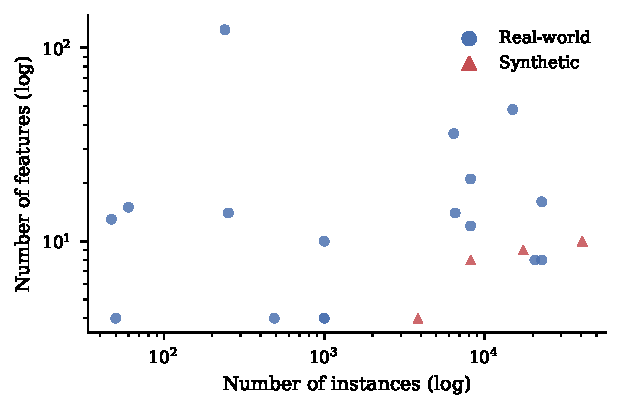
\includegraphics[width=0.62\textwidth]{figuras/fig_datasets.pdf}
\caption{Number of instances and number of features of the selected data sets (log scales).}
\label{fig:datasets}
\legend{Source: The Author}
\end{figure}

\section{Learning Algorithms and Implementation}
\label{sec:met-algoritmos}

The five algorithms described in Section~\ref{sec:fund-algoritmos} were used in
every scenario, through their scikit-learn implementations:
\texttt{LinearRegression} (LR), \texttt{KNeighborsRegressor} (KNN),
\texttt{DecisionTreeRegressor} (DT), \texttt{RandomForestRegressor} (RF), and
support vector regression (SVR). Outside the tuning scenario, all algorithms were
used with their default settings (for KNN, $k=5$ with the Euclidean distance;
for RF, 100 trees), and DT and RF received a fixed random seed so that differences between paired runs were not
caused by the randomness of tree construction.

Two implementation details concern SVR. First, because its regularization
parameter $C$ and its tolerance $\varepsilon$ are expressed in the scale of the
target, SVR was wrapped in a \texttt{TransformedTargetRegressor} that
standardizes the target inside each training fold and transforms predictions
back to the original scale before the metrics are computed; this transformation
is fitted only on training data in both pipelines and is therefore not a source
of leakage. Second, kernel SVR has a training cost that grows between
quadratically and cubically with the number of instances
\cite{chang2011}, which made it too slow for the largest data sets in the scenarios that do not
involve tuning. In the normalization, imputation, and
feature selection scenarios, SVR was thus trained with a linear model solved by
LIBLINEAR (\texttt{LinearSVR}, $C=1$, $\varepsilon=0.1$, $\varepsilon$-insensitive
loss) \cite{fan2008}, which optimizes the same objective as a linear-kernel SVR
at a cost that grows linearly with the data size. In the tuning scenario, in
which the kernel is one of the searched hyperparameters, the LIBSVM-based
\texttt{SVR} implementation was used.
% TODO (Vinicius): confirmar se as rodadas finais usaram os valores padrao das
% variaveis de ambiente (SVR_IMPL=linear, SVR_SCALE_Y=1, NUM_TRIALS=6) e se houve
% subamostragem do SVR (SVR_MAX_ROWS) no tuning. O texto acima assume os padroes.

\section{Leakage Scenarios}
\label{sec:met-cenarios}

The four scenarios are described below. Table~\ref{tab:cenarios} summarizes, for
each one, the validation protocol, the specific factor and its levels, and the
number of pairs obtained.

\begin{table}[htb]
\centering
\caption{Summary of the experimental setup of each leakage scenario.}
\label{tab:cenarios}
\small
\begin{tabular}{p{2.5cm}p{3.6cm}p{4.4cm}r}
\toprule
\textbf{Scenario} & \textbf{Validation} & \textbf{Specific factor (levels)} & \textbf{Pairs} \\
\midrule
Normalization & 6 $\times$ 4-fold CV & -- & 630 \\
Imputation & 6 $\times$ 4-fold CV & Imputer (mean, median, KNN) $\times$ missing rate (5, 10, 20, 30\%) & 7,560 \\
Feature selection & 6 $\times$ hold-out (80/20) & Percentile of features kept (1, 5, 10, 20\%) & 2,520 \\
Hyperparameter tuning & 6 $\times$ 4-fold CV (nested in the leakage-free pipeline) & -- & 630 \\
\bottomrule
\end{tabular}
\\[2pt]
\footnotesize Source: The Author. Pairs = 21 data sets $\times$ 5 algorithms $\times$ levels $\times$ 6 repetitions.
\end{table}

\subsection{Normalization}
\label{sec:met-normalizacao}

Features were standardized with the $z$-score transformation
(Equation~\ref{eq:zscore}), implemented by scikit-learn's
\texttt{StandardScaler}. In the leakage-free pipeline, the scaler is the first
step of a \texttt{Pipeline} object evaluated with $4$-fold CV, so that its means
and standard deviations are re-estimated on the three training folds of each
iteration. In the leakage-prone pipeline, the scaler is fitted once on the whole
data set, the standardized matrix is passed to the CV, and the pipeline evaluated
inside the CV has no scaling step. In each repetition $i$, both pipelines use the
same \texttt{KFold} partition (with shuffling and seed $i$), and the score of the
repetition is the average of the four test folds.

\subsection{Missing Value Imputation}
\label{sec:met-imputacao}

Since PMLB data sets are complete, missing values had to be introduced
artificially. To make the scenario closer to real data, a MAR mechanism was adopted, using
the masking procedure proposed by \citeonline{muzellec2020}, whose reference
implementation was adapted for this work. In this procedure, a random subset of
90\% of the features (at least one) is kept fully observed; each of the
remaining features receives missing values with probabilities given by a
logistic model of the observed features, whose random coefficients are
normalized and whose intercepts are adjusted so that the expected proportion of
missing entries in each affected feature equals the target missing rate. Four
rates were used: 5\%, 10\%, 20\%, and 30\%. The target column was never masked.
The incomplete data set is generated once per data set and missing rate, and is
shared by both pipelines and by all algorithms and imputers, so that every pair
sees exactly the same missing entries. Note that, by construction, only about
one tenth of the features are affected; for the many data sets with four to ten
features, this corresponds to a single incomplete feature.

Three imputers were compared: mean and median imputation
(\texttt{SimpleImputer}) and KNN imputation (\texttt{KNNImputer}, $k = 5$). In
the leakage-free pipeline, the imputer is the first step of the pipeline,
followed by the scaler and the regressor, and is refitted on the training folds
of each CV iteration. In the leakage-prone pipeline, the imputer is fitted and
applied to the complete incomplete matrix, after which the imputed data are
evaluated with the pipeline \emph{scaler $\rightarrow$ regressor}. As in the
normalization scenario, both pipelines are evaluated with the same $4$-fold
partitions in each of the six repetitions.

\subsection{Feature Selection}
\label{sec:met-selecao}

Feature selection was performed with a univariate filter, scikit-learn's
\texttt{SelectPercentile} with the $F$-statistic for regression
(\texttt{f\_regression}), keeping 1\%, 5\%, 10\%, or 20\% of the
highest-scoring features. These low percentiles were chosen on purpose: the fewer features are kept, the
more the result depends on the exact ranking of the features, and the more the
test instances can influence it.
Whenever a percentile would select less than one feature, it was raised to the
smallest value that keeps exactly one, and the same adjusted value was used in
both pipelines. As a consequence, the 1\% and 5\% levels keep a single feature in every
data set with up to 21 features, the data sets with four features keep a single
feature at all four levels, and only \texttt{505\_tecator} keeps more than one
feature at the 1\% level. Different levels may therefore correspond to the same
selection, a fact that must be considered when interpreting the results by level.

This scenario uses repeated hold-out instead of CV. In the leakage-prone
pipeline, the selector is fitted once on all instances, \emph{including their
target values}, and the reduced matrix is then split into training (80\%) and
test (20\%) sets. In the leakage-free pipeline, the split is made first and the
selector is fitted inside the pipeline on the training set only. In both cases
the pipeline continues with the scaler and the regressor, and the metrics are
computed on the predictions for the test set. Each of the six repetitions uses a
different random split (seed $i$), shared by both pipelines.

\subsection{Hyperparameter Tuning}
\label{sec:met-tuning}

Hyperparameters were tuned by exhaustive grid search (\texttt{GridSearchCV}).
The grids, listed in Table~\ref{tab:grades}, were kept small enough to make nested CV feasible on all data sets, but still
contain between four and fifteen
candidate configurations per algorithm. In the leakage-prone pipeline, a single
$4$-fold CV is used both to select the configuration and to report its
performance: for each metric, the reported value is the mean CV score of the
best configuration according to that same metric, which corresponds to the
common practice of reporting the best score found during the search. In the
leakage-free pipeline, the same search is embedded in a nested CV: the outer
$4$-fold CV, with exactly the same partitions as the leakage-prone pipeline,
provides the test folds, and an inner $4$-fold CV run on the training part of
each outer fold selects the configuration (by MSE), which is then refitted on
that training part and evaluated on the outer test fold. In both pipelines,
feature scaling is part of the pipeline being tuned.

\begin{table}[htb]
\centering
\caption{Hyperparameter grids used in the tuning scenario.}
\label{tab:grades}
\small
\begin{tabular}{lp{8.6cm}r}
\toprule
\textbf{Alg.} & \textbf{Grid} & \textbf{Configs.} \\
\midrule
LR  & \texttt{fit\_intercept} $\in$ \{True, False\}; \texttt{positive} $\in$ \{True, False\} & 4 \\
KNN & $k \in \{3, 5, 7, 9, 11\}$; distance $\in$ \{Euclidean, Manhattan\} & 10 \\
DT  & \texttt{max\_depth} $\in \{3, 5, 8, 10, \text{None}\}$ & 5 \\
RF  & \texttt{n\_estimators} $\in \{100, 200, 500\}$; \texttt{max\_depth} $\in \{3, 5, 8, 10, \text{None}\}$ & 15 \\
SVR & $C \in \{0.01, 0.1, 1, 10, 100\}$; kernel $\in$ \{linear, RBF\} & 10 \\
\bottomrule
\end{tabular}
\\[2pt]
\footnotesize Source: The Author
\end{table}

\section{Effect Measures and Statistical Analysis}
\label{sec:met-analise}

The four metrics of Section~\ref{sec:fund-regressao} were recorded for every
run. The analysis concentrates on $R^2$, which is comparable across data sets,
and uses RMSE as a complementary measure. For each pair, the effect of leakage is
quantified by
\begin{equation}
  \Delta R^2 = R^2_{\text{leak}} - R^2_{\text{no leak}}
  \qquad \text{and} \qquad
  \Delta\text{RMSE} = 100 \times \frac{\text{RMSE}_{\text{no leak}} - \text{RMSE}_{\text{leak}}}{\text{RMSE}_{\text{no leak}}}\;(\%).
  \label{eq:deltas}
\end{equation}
Both measures are oriented so that a \emph{positive} value means that leakage
made the model look better than it is: a higher $R^2$ or a lower RMSE. $\Delta$RMSE
is expressed as a percentage of the leakage-free RMSE to remove the dependence on
the scale of the target. A pair is considered a tie when
$\lvert \Delta R^2 \rvert \leq 10^{-9}$, a tolerance that absorbs floating-point
noise; the proportions of pairs in which leakage improved, did not change, or
worsened the estimate are reported for each scenario and algorithm.

Statistical tests follow the recommendations of \citeonline{demsar2006} and use
the data set as the unit of analysis. For each scenario and algorithm, the
$\Delta R^2$ of all pairs of a data set (across repetitions and levels of the
specific factor) are averaged, producing 21 values, one per data set. The
two-sided Wilcoxon signed-rank test is applied to these values to test whether
the median effect differs from zero, and the five $p$-values of each scenario
(one per algorithm) are adjusted with the Holm procedure. Results are considered
significant at $\alpha = 0.05$ after adjustment. Testing each configuration separately would be less informative, since with six
pairs the smallest possible two-sided $p$-value is $0.031$; at that level, the number of configurations in
which leakage improved the estimate in all six repetitions is reported instead,
as a descriptive measure of consistency.

To answer RQ3, the Friedman test is applied, in each scenario, to the
per-data-set mean $\Delta R^2$ of the five algorithms, testing whether some
algorithms are systematically more affected than others. To answer RQ4, the
Spearman correlation is computed between the per-data-set mean $\Delta R^2$
(averaged over algorithms) and the number of instances ($n$), the number of
features ($d$), and the ratio $d/n$. The analysis scripts were written in Python
with pandas and SciPy, and all numbers reported in Chapter~\ref{cap:resultados}
are produced by the script \texttt{tcc/scripts/gerar\_tabelas\_figuras.py}
directly from the raw result files.
